%versi 2 (8-10-2016) 
\chapter{Pendahuluan}
\label{chap:intro}

\section{Latar Belakang}
\label{sec:label}

Ruang Terbuka Hijau merupakan suatu ruang terbuka di kawasan perkotaan yang didominasi tutupan lahannya oleh unsur hijau (vegetasi) serta memiliki fungsi antara lain sebagai area untuk rekreasi, sosial budaya, estetika, ekologis dan dapat memberikan nilai ekonomis bagi perkembangan suatu wilayah perkotaan (lihat Gambar \ref{fig:rth}). Definisi RTH sendiri dalam pasal 1 UU No.26/2007 tentang Penataan Ruang adalah area memanjang/jalur dan/atau mengelompok, yang penggunaannya lebih bersifat terbuka, tempat tumbuh tanaman, baik yang tumbuh secara alamiah maupun yang sengaja ditanam. Pada pasal 29 disebutkan bahwa ruang terbuka hijau terdiri dari ruang terbuka hijau publik dan ruang terbuka hijau privat, dimana proporsi ruang terbuka hijau kota paling sedikit 30\% dari luas wilayah kota, sedangkan proporsi ruang terbuka hijau publik paling sedikit 20\% dari luas wilayah kota. %jgn lupa referensi

\begin{figure}[h]
	\centering
	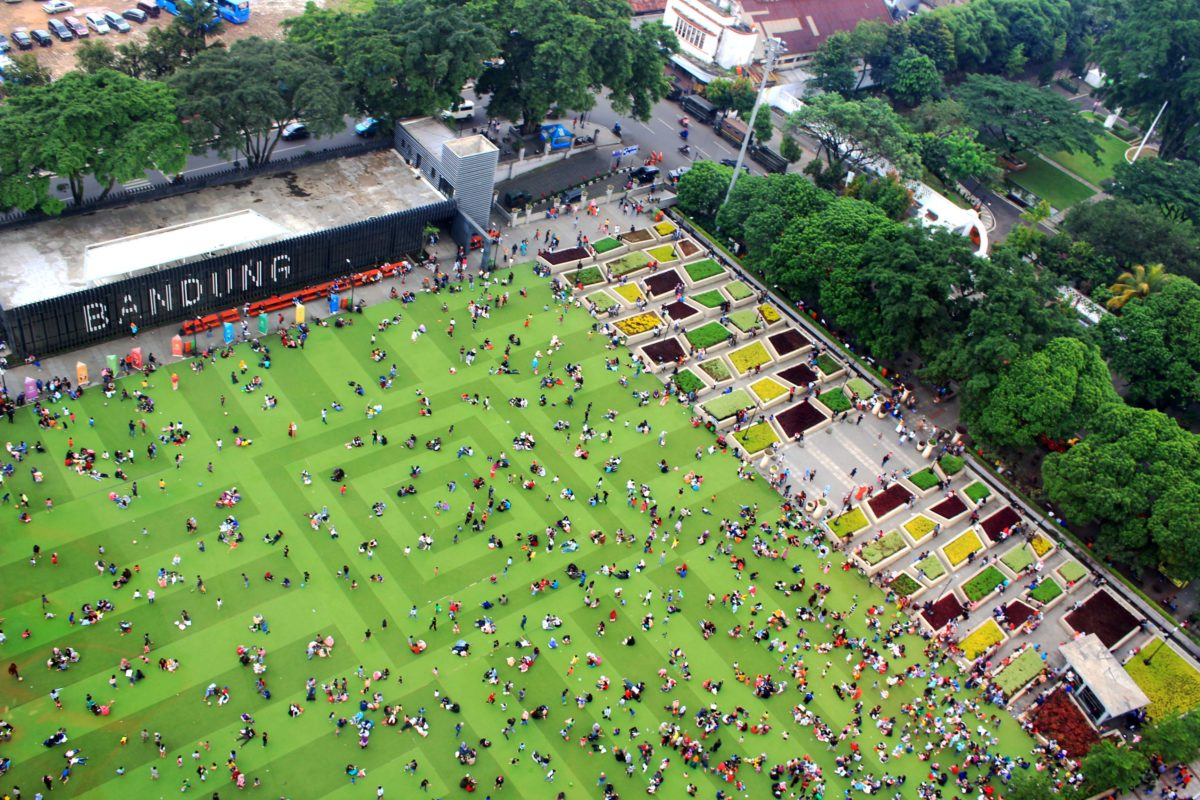
\includegraphics[width=0.7\textwidth]{ruang terbuka hijau.jpg}
	\caption[RTH]{Contoh Ruang Terbuka Hijau\footnote{Ilustrasi ruang terbuka hijau\url{https://www.rth.bandung.go.id/}}}
	\label{fig:rth}
\end{figure}


Pemanfaatan citra satelit merupakan sebuah cara agar dapat mengetahui luas RTH pada suatu kota. Citra Satelit adalah gambaran dari permukaan bumi yang didapatkan langsung dari satelit. Oleh karena itu, citra satelit dapat digunakan dalam mengidentifikasi RTH yang mana terdapatnya banyak pepohonan pada suatu wilayah. Perhitungan juga dapat dilakukan pada citra satelit ,dan hasil dari perhitungan luas RTH pada suatu wilayah diharapkan dapat memberikan dorongan untuk peningkatan dalam penghijauan agar dapat digunakan oleh pemerintah dalam merancang dan meningkatkan penghijauan di berbagai wilayah di Indonesia.

Penelitian yang dilakukan oleh Juan A. Kusjadi yaitu mengimplementasikan program untuk mengumpulkan, menyiapkan, dan menganalisis data
citra satelit kelurahan dari beberapa kota/kabupaten di Indonesia menggunakan Hadoop MapReduce. Data kemudian disimpan pada sistem data lake yang telah dibuat pada Hadoop HDFS. Data hasil analisis dan perhitungan luas RTH juga sudah dilakukan evaluasi dengan nilai sesungguhnya\cite{juan:22:pengumpulan}. Data hasil penelitian akan digunakan sebagai penunjang dalam pembuatan halaman web. 

Pada Skripsi ini, akan dibangun sebuah halaman web yang interaktif yaitu pemvisualisasian dari hasil penelitian area hijau Kota Bandung\cite{juan:22:pengumpulan}. Visualisasi adalah rekayasa dalam pembuatan gambar, diagram atau animasi untuk penampilan suatu informasi dalam penjelasan lain visualisasi adalah konversi data ke dalam format visual atau tabel sehingga karakteristik dari data dan relasi diantara item data atau atribut dapat di analisis atau dilaporkan, dan visualisasi data adalah satu dari yang teknik paling baik dan menarik untuk eksplorasi data. Manusia memiliki kemampuan membangun yang baik untuk menganalisis sejumlah besar informasi yang dipresentasi secara visual. Ia dapat mendeteksi pola umum dan trend, pencilan dan pola yang tidak umum. Oleh karena itu, dengan dikembangkannya halaman web ini memiliki tujuan agar para pengguna dapat mengetahui informasi yang terdapat pada kelurahan. Informasi yang terdapat pada halaman website berupa nama kelurahan, luas wilayah kelurahan, gambar dari keluruhan/kecamatan, dll. Informasi yang terkumpul akan digunakan untuk mengembangkan halaman web.
%Pressman, Roger S. 2002.”Rekayasa Perangkat Lunak (Pendekatan Praktis).” Yogyakarta : Andi


Halaman web yang akan dikembangkan harusnya dapat diakses melalui komputer atau laptop. Dalam pengembangan halaman web pemvisualisasi area hijau kota Bandung akan dibantu pembuatannya dengan menggunakan \emph{Framework} Laravel. Penggunaan \textit{Framework} Laravel untuk memudahkan pengembang untuk membangun halaman web, sehingga pengguna yang akan mengakses halaman web akan dimudahkan dalam melihat informasi kelurahan dengan cepat. 

Laravel merupakan \textit{framework} PHP yang menekankan pada kesederhanaan dan flesksibelitas pada desainnya. Keunggulan ini didapatkan karena Laravel menggunakan konsep MVC (Model View Controller). Model pada Laravel berguna untuk membantu pengembang berinteraksi dengan database mengunakan \textit{syntax migration} yang merupakan bawaan dari Laravel. Dengan \textit{migration}, pengembangan dapat dengan mudah untuk melakukan modifikasi sebuah database pada sebuah platform secara independen karena implementasi skemas \textit{database} yang direpresentasikan dalam sebuah class. View pada Laravel akan menjadi wadah tampilan website (\textit{frond-end}). Dan Controller yang berfungsi untuk merespon setiap request yang ada pada website sehingga setiap fungsi yang ada akan berfungsi sebagaimana mestinya. Dengan berbagai kemudahan dan fitur yang ada pada Laravel inilah yang membuat pemngembang ingin menggunakannya dalam membangun halaman web pemvisualisasian area hijau kelurahan kota Bandung.


Dalam proses pengembangan halaman web tentu saja dibutuhkan sebuah data. Data yang akan digunakan dalam pembentukan halaman web berupa gambar dari kelurahan di Kota Bandung. Tidak hanya berupa gambar dari kelurahan tetapi juga berupa luas area wilayah untuk mengetahui besar wilayah kelurahan, mengetahui luas wilayah hijau kelurahan, dan melihat kebutuhan area hijau terhadap kelurahan di Kota Bandung. Perhitungan luas wilayah, luas wilayah hijau, dan kebutuhan area hijau telah dilakukan perhitungan untuk setiap kelurahan yang ada. 

\begin{figure}[H]
	\centering
	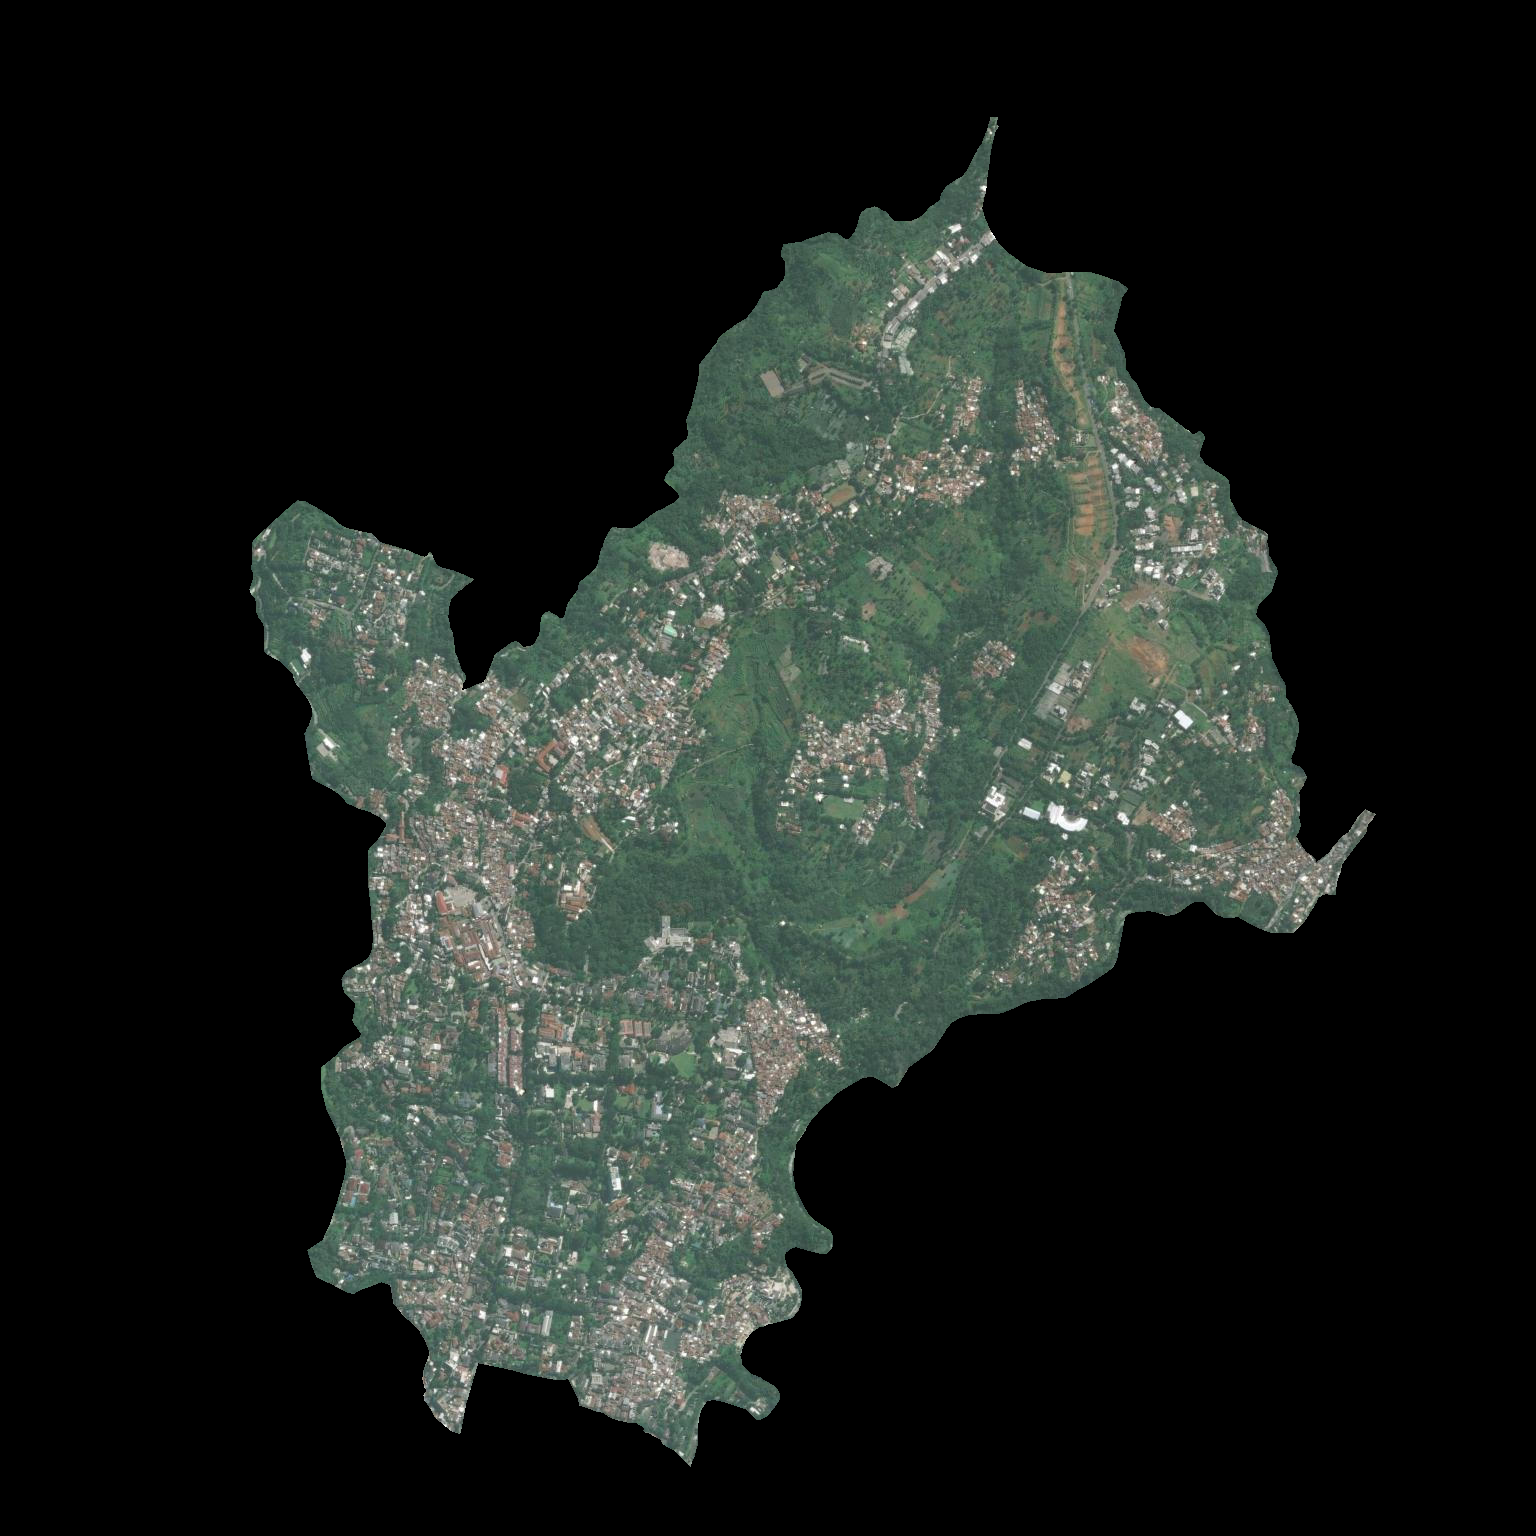
\includegraphics[width=0.6\textwidth]{Gambar/Ciumbuleuit.png}
	\caption{Kelurahan Ciumbuleuit}
	\label{fig:ciumbuleuit}
\end{figure}

Contoh gambar dari hasil penelitian Juan A. Kusjadi dapat dilihat pada gambar \ref{fig:ciumbuleuit} yang mana merupakan hasil proses pengambilan gambar sebuah kelurahan Ciumbuleuit yang telah disimpan pada Hadoop HDFS. Proses pengambilan gambar dilakukan dengan menggunakan bahasa pemrograman Python\footnote{Python adalah bahasa pemrograman yang banyak digunakan dalam aplikasi web, pengembangan perangkat lunak, ilmu data, dan \textit{machine learning} (ML). Developer menggunakan Python karena efisien dan mudah dipelajari serta dapat dijalankan di berbagai platform.}. Berbagai macam \textit{library} yang dapat digunakan pada bahasa pemrograman Python dalam membantu pengembangan laman web, diantaranya menggunakan \textit{Python PIL(Pillow)} yang berguna untuk menggabungkan gambar, dan \textit{library} base 64 yang digunakan dalam melakukan peng-\textit{decode}-an teks yang merupakan sebuah \textit{tile} gambar kelurahan.

Hasil dari pemvisualisasi ruang terbuka hijau kelurahan pada kota Bandung akan menjadi sebuah halaman website yang interaktif yang dapat membandingkan kelurahan sesuai dengan masukan oleh pengguna. Dengan dikembangkan halaman website ini maka pengguna dapat memenuhi kebutuhan tempat tinggal bagi masyarakat agar dapat beraktivitas dengan normal dan mendapatkan kadar oksigen yang merata. 

\section{Rumusan Masalah}
\label{sec:rumusan}
Berdasarkan deskripsi dan latar belakang yang sudah dibahas bahwa rumusan masalah yang muncul adalah sebagai berikut:

\begin{itemize}
	\item Bagaimana membuat sebuah halaman website interaktif yang dapat membandingkan data dua buah kelurahan Kota Bandung?
	\item Bagaimana cara pengguna untuk membandingkan atribut-atribut Citra Satelit dari kelurahan Kota Bandung?
	\item Bagaimana cara mengekstraksi data citra satelit pada HDFS ke \textit{local directory}?	
\end{itemize}

\section{Tujuan}
\label{sec:tujuan}
Tujuan dari skripsi ini adalah:
\begin{enumerate}
	\item Membuat sebuah halaman website interaktif yang dapat membandingkan dua lokasi kelurahan.
	\item Pengguna dapat memilih kelurahan untuk sisi kiri dan kanan, untuk membandingkan atributnya.
	\item Data citra satelit yang didapatkan akan digunakan untuk memenuhi kebutuhan pada laman web yang akan dibangun.
\end{enumerate}


\section{Batasan Masalah}
\label{sec:batasan}
Tidak memiliki batasan masalah

\section{Metodologi}
\label{sec:metlit}
Metodologi yang akan digunakan dalam pembuatan skripsi adalah:
\begin{enumerate}
	\item Melakukan survei kepada Fritz H. Hutapea SKom dan Juan A. Kusjadi terkait penenilitiannya
	\item Melakukan pengumpulan data hasil penelitian
	\item Mempelajari ekstraksi data citra satelit yang disimpan pada HDFS
	\item Mempelajari bahasa pemrograman php, html, css dan cara menggunakan \emph{framework} laravel.
	\item Mempelajari kebutuhan laman web.
	\item Melakukan analisis kebutuhan laman web.
	\item Melakukan perancangan antar muka laman web.
	\item Membangun laman web bedasarkan \emph{framework} Laravel.
	\item Melakukan pengujian pada laman web.
	\item Menulis dokumen skripsi.
\end{enumerate}

\section{Sistematika Pembahasan}
\label{sec:sispem}
%Rencananya Bab 2 akan berisi petunjuk penggunaan template dan dasar-dasar \LaTeX.
%Mungkin bab 3,4,5 dapt diisi oleh ketiga jurusan, misalnya peraturan dasar skripsi atau pedoman penulisan, tentu jika berkenan.
%Bab 6 akan diisi dengan kesimpulan, bahwa membuat template ini ternyata sungguh menghabiskan banyak waktu.

Skripsi ini disusun dalam beberapa bab secara sistematis sebagai berikut:
\begin{itemize}
	\item \textbf{Bab 1 Pendahuluan} \\ 
	Berisikan tentang latar belakang, rumusan masalah, tujuan, batasan masalah, metodologi, dan sistematika pembahasan.
	\item \textbf{Bab 2 Landasan Teori} \\ 
	Berisikan tentang dasar-dasar dari teori-teori yang digunakan dalam membangun halaman web seperti \textit{Command-line interface}, \textit{Hadoop Distributed File System}, \textit{Python} beserta \textit{library}-nya, Base 64, dan \textit{Framework}.
	\item \textbf{Bab 3 Analisis} \\ 
	Pada bab ini akan menjelaskan proses pembentukan gambar didalamannya terdapat bagaimana cara pengunduhan teks, pengkonversian baris menjadi gambar, dan menggabungkan gambar. Juga terdapat analisis kebutuhan perangkat lunak.
	\item \textbf{Bab 4 Perancangan} \\
	Berisikan tetang penjelaskan mengenai perancangan yang digunakan dalam membangun perangkat lunak.
	\item \textbf{Bab 5 Implementasi dan Pengujian} \\
	Bab ini membahasan tentang pengimplementasian rancangan antarmuka agar dapat menampilkan perbandingan visual antara dua kelurahan di kota Bandung. Juga akan membahas tentang pengujian fungsional dan pengujian eksperimental.
	\item \textbf{Bab 6 Kesimpulan dan Saran} \\
	Bab ini berisikan kesimpulan dari hasil pengerjaan skripsi, dan saran untuk pengembangan selanjutnya.
	
	
\end{itemize}
